%Chapter 4

\renewcommand{\thechapter}{4}

\chapter{Results}

\section{Simulations}
\label{sec: s4.1}
Determining results for the simulations was an iterative process. The first batch of simulations helped us to 
determine which variables did not influence the results and which had more effects. During the second batch we were 
able to test more scenarios to obtain more useful data by comparing charge output to cost. Analysis of the second 
batch allowed us to run a third smaller batch of simulations to obtain more accurate results for our final 
recommendations.

\subsection{Batch 1}
\subsubsection{Inputs}
For the of simulations the minimum and maximum predicted values for each variable based on the Society of Automotive 
Engineering Standard J2954 \cite{noauthor_j2954_nodate}. The voltage coming from the road was chosen based on the minimum and 
maximum voltages that solar panels come in, which is 96 and 100 volts respectively.  For the wire gauge, only 
standard wire gauge sizes were used since they come in standard sizes. The number of turns in the road coils, 
the number of turns was determined based on the amount in a pancake coil which is anywhere between 413 and 566 turns. 
The radius of the road coils was taken to be between 2.7 m and 3.7 m since this is the average width of low volume 
road width and standard lane width. 

The inputs for the coils that will be in the car is different since they will be the receiving coils. 
The wire gauge will still be the standard size for wire gauges, but the number of turns will be 229 for the 
minimum and 321 for the maximum. The radius for the coils will be 1.5 m for the maximum and 2.1 for the minimum 
and this comes from the average width of a compact car versus the average width of a full-size SUV since this 
will be the ranges of cars that will be on the road. 

The orientation of the coils in the simulation was also determined from research. For the height of the coils 
above the ground, the range of 0 to 0.5 m was chosen since the average vehicle ground clearance is 0.25 m. 
The Society of Automotive Engineers states that the most efficient spacing of coils would be no more than 18 cm 
between the closest parts \cite{noauthor_j2954_nodate}. Using this would mean that the spacing input for the simulation would 
be two times the radius of the coil for the minimum and two times the radius of the coil plus 0.3 m for the maximum. 
The velocity that is inputted into the simulation was 18 m/s for the minimum and 36 m/s for the maximum since this 
is the low highway speed to high highway speed. 

\begin{itemize}
    \item V = [96 600] [V]
    \item wireGauge = [8] []
    \item turns = [410 570] []
    \item radius = [2.5 4] [m]
    \item wireGauge\_car = [12] []
    \item turns\_car = [230 320] []
    \item radius\_car = [1.5 2] [m]
    \item height = [0 .5] [m]
    \item spacing = [0 .36] [m]
    \item velocity = [18 36] [m/s]
\end{itemize}

\subsubsection{Outputs}
The outputs of our simulation were compiled into graphs using analysis.py. Each graph shows the charge graphed 
against each variable. Outputs with the same inputs besides the varied value are connected by lines in order to 
show how a nearly identical simulation is affected by changing that variable. The first batch of simulations 
showed that velocity is not a factor in charge, which makes sense since the field is the same, see Figure \ref{fig: f20}. 
Figure \ref{fig: f13} shows the output charge versus voltage when the first simulation was run. This graph shows that as the 
voltage increases the output charge increases linearly. Figure \ref{fig: f14} shows the output charge versus the number of turns. 
As the number of turns increase the output charge decreases slowly. This shows that increasing the number of turns 
does not optimize the charge gained. Figure \ref{fig: f15} shows that output charge is only slightly dependent on the radius of 
the coil in the road since the slope is only increasing slightly. 
 	 
\begin{figure}
    \begin{center}
    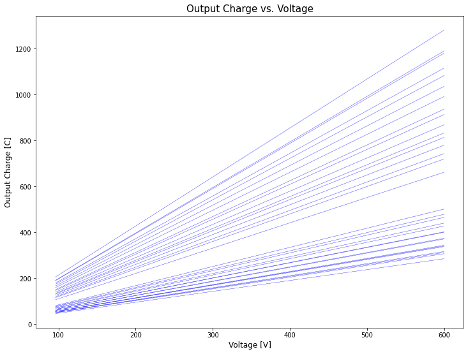
\includegraphics[width=3in]{fig13.png}
    \end{center}
    \renewcommand{\baselinestretch}{1}
    \small\normalsize
    \begin{quote}
    \caption[Batch 1 Output Charge vs. Voltage]{Batch 1 Output Charge vs. Voltage} \label{fig: f13}
    \end{quote}
\end{figure}

\begin{figure}
    \begin{center}
    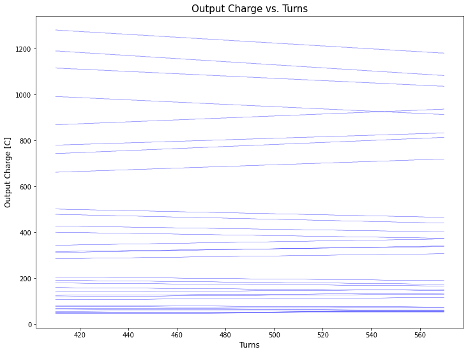
\includegraphics[width=3in]{fig14.png}
    \end{center}
    \renewcommand{\baselinestretch}{1}
    \small\normalsize
    \begin{quote}
    \caption[Batch 1 Output Charge vs. Turns]{Batch 1 Output Charge vs. Turns} \label{fig: f14}
    \end{quote}
\end{figure}

\begin{figure}
    \begin{center}
    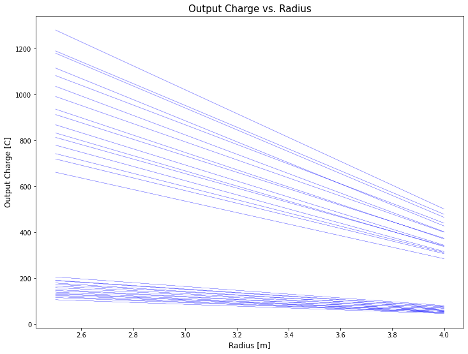
\includegraphics[width=3in]{fig15.png}
    \end{center}
    \renewcommand{\baselinestretch}{1}
    \small\normalsize
    \begin{quote}
    \caption[Batch 1 Output Charge vs. Radius]{Batch 1 Output Charge vs. Radius} \label{fig: f15}
    \end{quote}
\end{figure}

\begin{figure}
    \begin{center}
    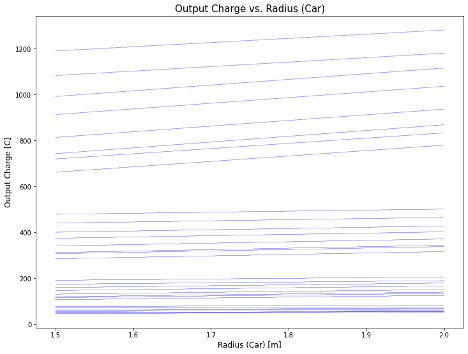
\includegraphics[width=3in]{fig16.png}
    \end{center}
    \renewcommand{\baselinestretch}{1}
    \small\normalsize
    \begin{quote}
    \caption[Batch 1 Output Charge vs. Radius of Coil on Car]{Batch 1 Output Charge vs. Radius of Coil on Car} \label{fig: f16}
    \end{quote}
\end{figure}

As for the coils in the car, Figure \ref{fig: f16} shows that the car coils radius has a bigger effect than the road coils 
radius on the output velocity. As the coils in the car start getting a bigger radius, the output charge decreases, 
so the coils in the car want to have a radius on the smaller side to optimize output charge. 
Figure \ref{fig: f17} shows that the number turns in the coil of the car increases the output charge. 
Figure \ref{fig: f18} shows that the height decreases the output charge goes down. As expected, as the spacing in the road 
increases, the output charge decreases as shown in Figure \ref{fig: f19}. 

\begin{figure}
    \begin{center}
    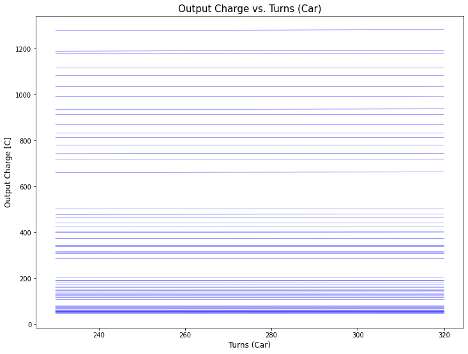
\includegraphics[width=3in]{fig17.png}
    \end{center}
    \renewcommand{\baselinestretch}{1}
    \small\normalsize
    \begin{quote}
    \caption[Batch 1 Output Charge vs. Turns of Coil on Car	]{Batch 1 Output Charge vs. Turns of Coil on Car} \label{fig: f17}
    \end{quote}
\end{figure}

\begin{figure}
    \begin{center}
    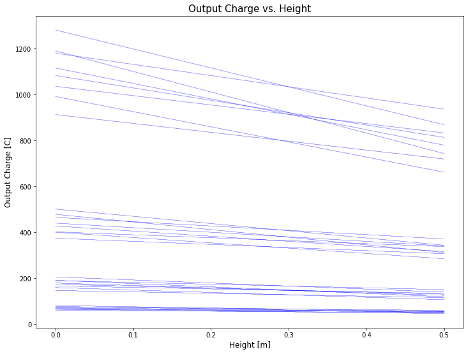
\includegraphics[width=3in]{fig18.png}
    \end{center}
    \renewcommand{\baselinestretch}{1}
    \small\normalsize
    \begin{quote}
    \caption[Batch 1 Output Charge vs. Height]{Batch 1 Output Charge vs. Height } \label{fig: f18}
    \end{quote}
\end{figure}

\begin{figure}
    \begin{center}
    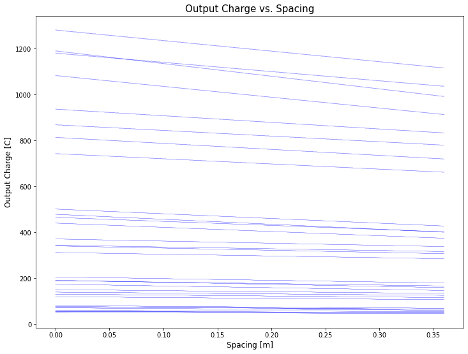
\includegraphics[width=3in]{fig19.png}
    \end{center}
    \renewcommand{\baselinestretch}{1}
    \small\normalsize
    \begin{quote}
    \caption[Batch 1 Output Charge vs. Spacing of Coils on Road]{Batch 1 Output Charge vs. Spacing of Coils on Road} \label{fig: f19}
    \end{quote}
\end{figure}

\begin{figure}
    \begin{center}
    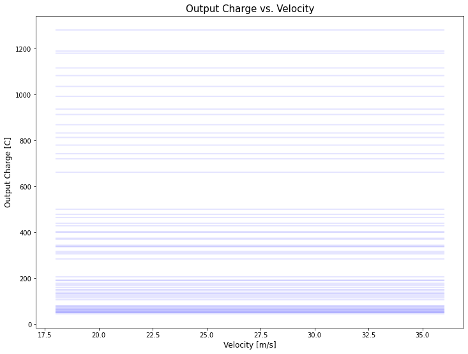
\includegraphics[width=3in]{fig20.png}
    \end{center}
    \renewcommand{\baselinestretch}{1}
    \small\normalsize
    \begin{quote}
    \caption[Batch 1 Output Charge vs. Velocity]{Batch 1 Output Charge vs. Velocity} \label{fig: f20}
    \end{quote}
\end{figure}

\subsection{Batch 2}
\subsubsection{Inputs}
Based on the outputs from Batch 1 the inputs were updated for a more refined set of simulations. 
We added a second option for both wire gauges in order to determine trends in those variables. 
In voltage, turns, radius, car turns, and car radius we added more values in the same ranges. 
For velocity we used 30 m/s because we found that velocity does not influence the charge output over the same 
distance. For height and spacing we replaced values with more realistic values of height and spacing in the original 
range. Below are the inputs for Batch 2, resulting in over 24,000 data points.

\begin{itemize}
    \item V = [100 250 450 600] [V]
    \item wireGauge = [6 8] []
    \item turns = [410 460 510 560] []
    \item radius = [1 2 3 4] [m]
    \item wireGauge\_car = [8 12] []
    \item turns\_car = [230 260 290 320] []
    \item radius\_car = [1.5 1.7 1.9 2.1] [m]
    \item height = [.15 .3] [m]
    \item spacing = [0 .18 .36] [m]
    \item velocity = [30] [m/s]
\end{itemize}

\subsubsection{Outputs}
Because Batch 2 has many more data points, we were able to observe more about the trends in the outputs. 
One important observation is that some variables do not impact cost of infrastructure, so optimal values 
for these can be as large as is reasonable for the physical configuration. These include wire gauge of the car 
coil, turns of the car coil, radius of the car coil, and height. Therefore, for Batch 3 we used only the values 
for these variables that correspond to the largest charge outputs. Other variables are worth looking into further. 
Voltage has a direct relationship with cost so for Batch 3 we used the value with the smallest corresponding 
cost/charge output, which is 100 V. Wire gauge has a constant relationship with cost, so we chose the largest 
charge value, which corresponds to 6-gauge wire.  Turns showed an interesting charge output so for Batch 3 we 
retested all values. Radius has a direct relationship with charge, however it experiences a huge drop off in output 
as radius increases, so it is worth a larger cost. Therefore, for Batch 3 we used only 1 m radius coils. 
For spacing, the trend is not increasing or decreasing for the entire time. For Batch 3, we tried more inputs 
in order to determine a better idea of the charge and cost correlations. We didn’y test spacing at 0 m because 
it clearly did not give a good charge output. See graphs below for each variable, excluding velocity as explained 
previously, for output charge, cost, and cost/charge. The graphs in Batch 2 (Figures \ref{fig: f21} through \ref{fig: f29}) are made in the same way as Batch 1, 
but there are additional graphs that graph cost vs. each variable as well as cost/charge vs. each variable.

\begin{figure}
    \begin{center}
    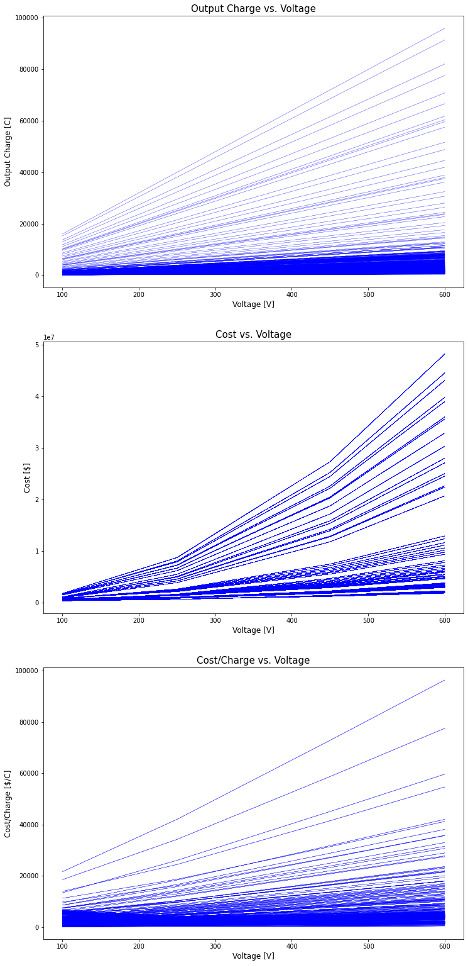
\includegraphics[width=3in]{fig21.png}
    \end{center}
    \renewcommand{\baselinestretch}{1}
    \small\normalsize
    \begin{quote}
    \caption[Batch 2 Voltage Trends]{Batch 2 Voltage Trends} \label{fig: f21}
    \end{quote}
\end{figure}

\begin{figure}
    \begin{center}
    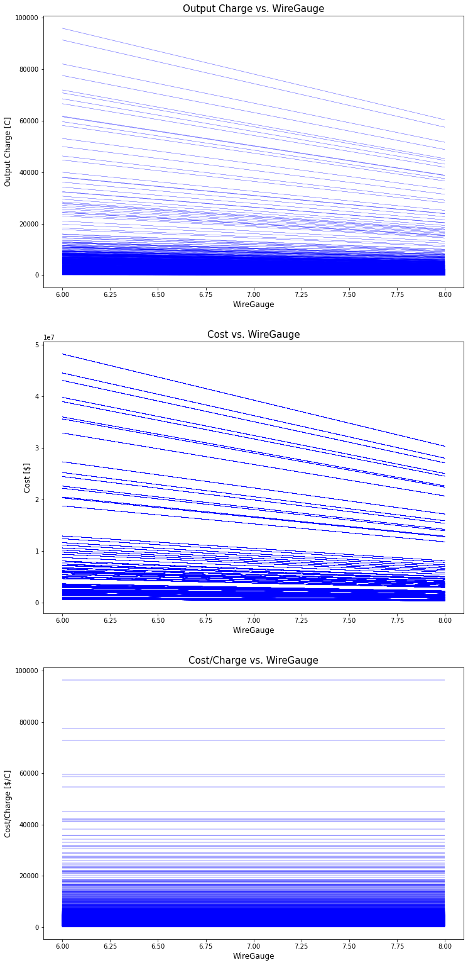
\includegraphics[width=3in]{fig22.png}
    \end{center}
    \renewcommand{\baselinestretch}{1}
    \small\normalsize
    \begin{quote}
    \caption[Batch 2 WireGauge Trends]{Batch 2 WireGauge Trends} \label{fig: f22}
    \end{quote}
\end{figure}

\begin{figure}
    \begin{center}
    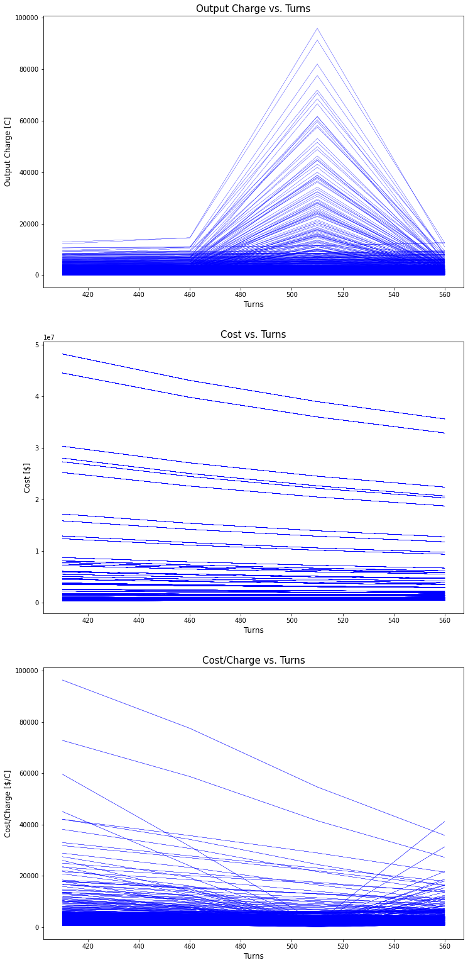
\includegraphics[width=3in]{fig23.png}
    \end{center}
    \renewcommand{\baselinestretch}{1}
    \small\normalsize
    \begin{quote}
    \caption[Batch 2 Turns Trends]{Batch 2 Turns Trends} \label{fig: f23}
    \end{quote}
\end{figure}

\begin{figure}
    \begin{center}
    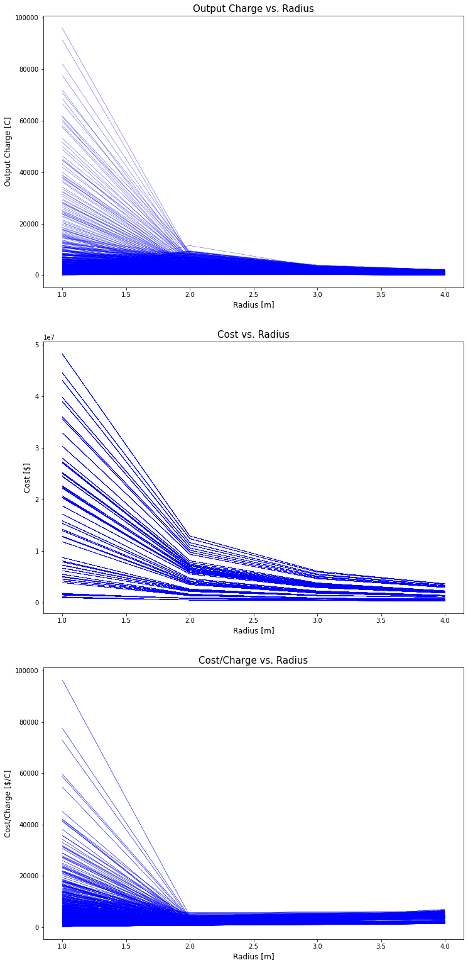
\includegraphics[width=3in]{fig24.png}
    \end{center}
    \renewcommand{\baselinestretch}{1}
    \small\normalsize
    \begin{quote}
    \caption[Batch 2 Radius Trends]{Batch 2 Radius Trends} \label{fig: f24}
    \end{quote}
\end{figure}

\begin{figure}
    \begin{center}
    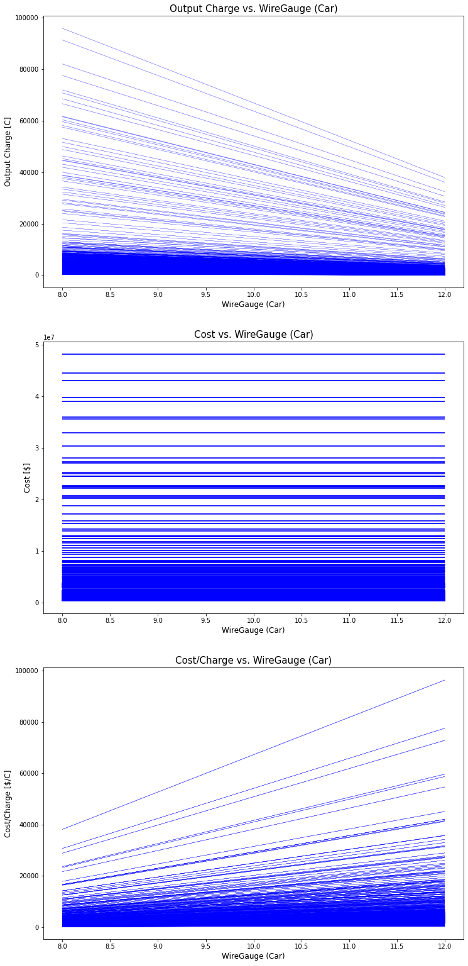
\includegraphics[width=3in]{fig25.png}
    \end{center}
    \renewcommand{\baselinestretch}{1}
    \small\normalsize
    \begin{quote}
    \caption[Batch 2 WireGauge (Car) Trends	]{Batch 2 WireGauge (Car) Trends	} \label{fig: f25}
    \end{quote}
\end{figure}

\begin{figure}
    \begin{center}
    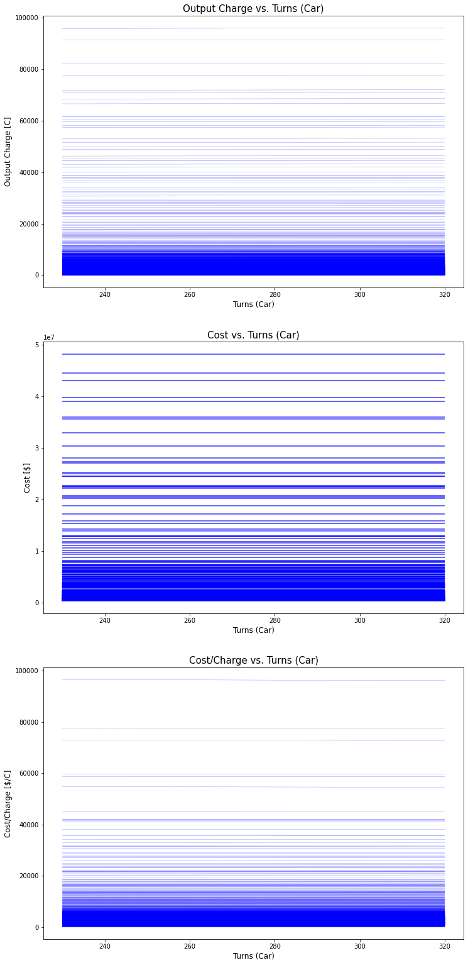
\includegraphics[width=3in]{fig26.png}
    \end{center}
    \renewcommand{\baselinestretch}{1}
    \small\normalsize
    \begin{quote}
    \caption[Batch 2 Turns (Car) Trends]{Batch 2 Turns (Car) Trends} \label{fig: f26}
    \end{quote}
\end{figure}

\begin{figure}
    \begin{center}
    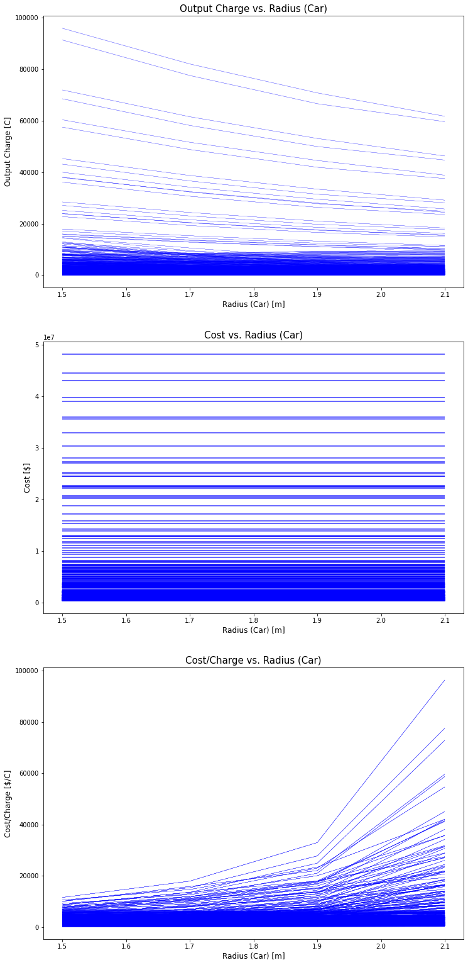
\includegraphics[width=3in]{fig27.png}
    \end{center}
    \renewcommand{\baselinestretch}{1}
    \small\normalsize
    \begin{quote}
    \caption[Batch 2 Radius (Car) Trends]{Batch 2 Radius (Car) Trends} \label{fig: f27}
    \end{quote}
\end{figure}

\begin{figure}
    \begin{center}
    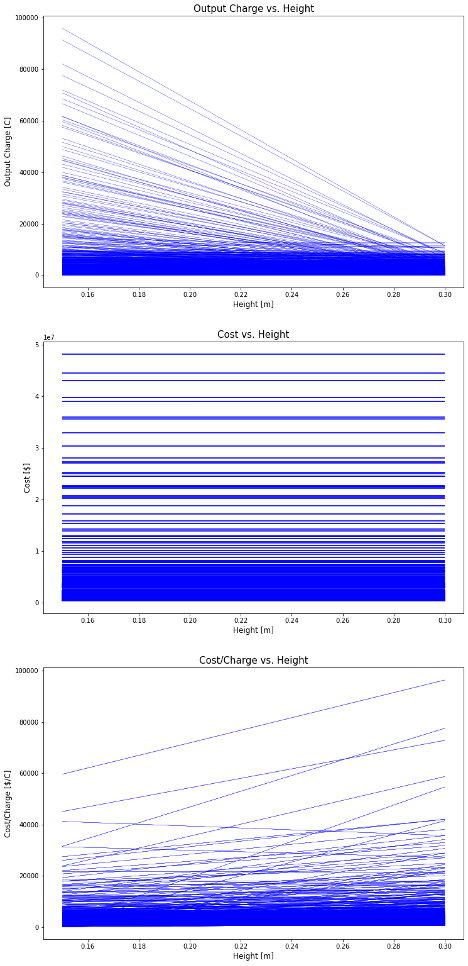
\includegraphics[width=3in]{fig28.png}
    \end{center}
    \renewcommand{\baselinestretch}{1}
    \small\normalsize
    \begin{quote}
    \caption[Batch 2 Height Trends]{Batch 2 Height Trends} \label{fig: f28}
    \end{quote}
\end{figure}

\begin{figure}
    \begin{center}
    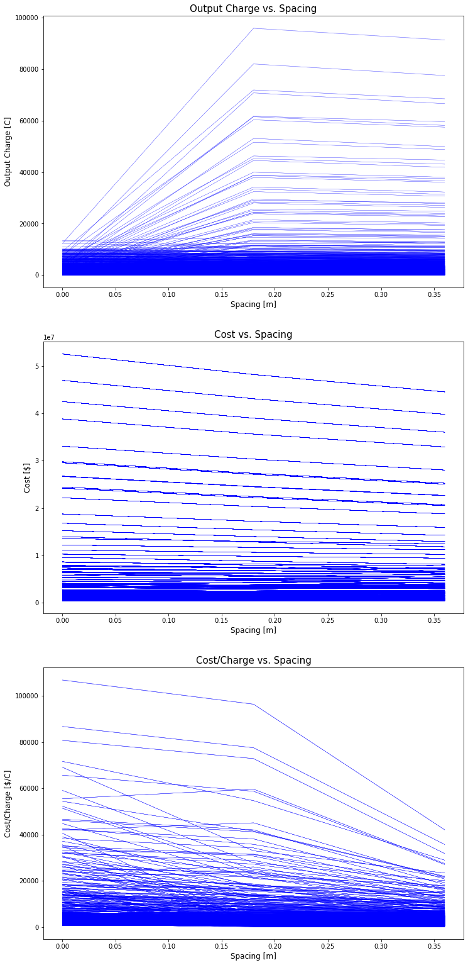
\includegraphics[width=3in]{fig29.png}
    \end{center}
    \renewcommand{\baselinestretch}{1}
    \small\normalsize
    \begin{quote}
    \caption[Batch 2 Spacing Trends]{Batch 2 Spacing Trends} \label{fig: f29}
    \end{quote}
\end{figure}

\subsection{Batch 3}
\label{sec: s4.1.3}
\subsubsection{Inputs}
The purpose of Batch 3 was to obtain more accurate values for charge. This is possible using smaller values of 
the increment (and therefore distanceStep) and filamentStep. We decreased the increment by a factor of 2 and 
increased the filament step by a factor of 10. This makes the mesh grid much finer, so many more calculations 
need to be done, which takes much longer. Therefore, we ran only 17 scenarios. We ran 16 scenarios to obtain 
more accurate values for economical configurations as determined from Batch 2 outputs. The inputs for the 
scenarios are below. 

\begin{itemize}
    \item V = [100] [V]
    \item wireGauge = [6] []
    \item turns = [410 460 510 560] []
    \item radius = [1] [m]
    \item wireGauge\_car = [8] []
    \item turns\_car = [320] []
    \item radius\_car = [1.5] [m]
    \item height = [.15] [m]
    \item spacing = [.09 .18 .27 .36] [m]
    \item velocity = [30] [m/s]
\end{itemize}

We ran one additional scenario that produced the largest overall charge in Batch 2. In case there is not an 
economical configuration that produces a reasonable charge output, it would be valuable to determine if any 
configuration would produce a reasonable charge output. The input for this scenario is below. 

\begin{itemize}
    \item V = [600] [V]
    \item wireGauge = [6] []
    \item turns = [510] []
    \item radius = [1] [m]
    \item wireGauge\_car = [8] []
    \item turns\_car = [320] []
    \item radius\_car = [1.5] [m]
    \item height = [.15] [m]
    \item spacing = [.09] [m]
    \item velocity = [30] [m/s]
\end{itemize}

\subsubsection{Outputs}
From analysis of the Batch 3 results, we can see that cost effectiveness decreases as both turns and spacing 
increase, so the most economical scenario corresponds to 410 turns and .09 spacing. This configuration output 
2142.7 C for 1600 m. See the Figures \ref{fig: f30} and \ref{fig: f31} below for the data trends.

\begin{figure}
    \begin{center}
    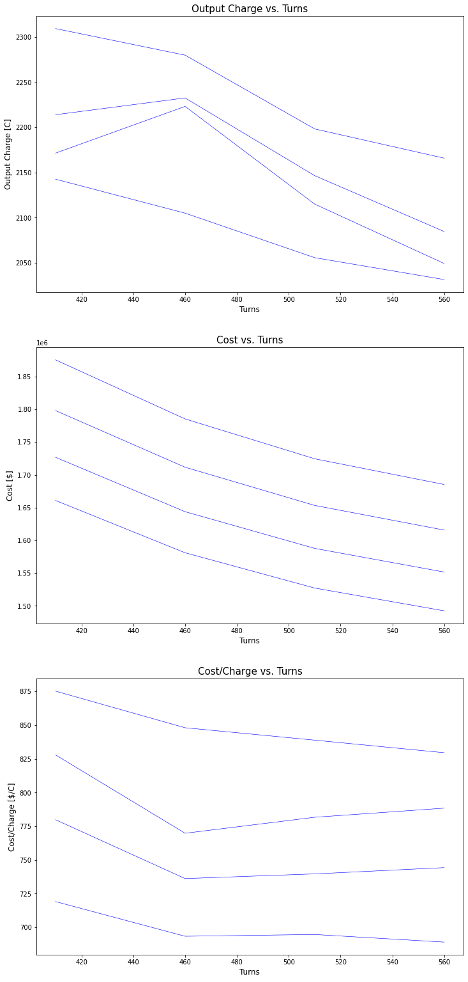
\includegraphics[width=3in]{fig30.png}
    \end{center}
    \renewcommand{\baselinestretch}{1}
    \small\normalsize
    \begin{quote}
    \caption[Batch 3 Turns Trends]{Batch 3 Turns Trends} \label{fig: f30}
    \end{quote}
\end{figure}

\begin{figure}
    \begin{center}
    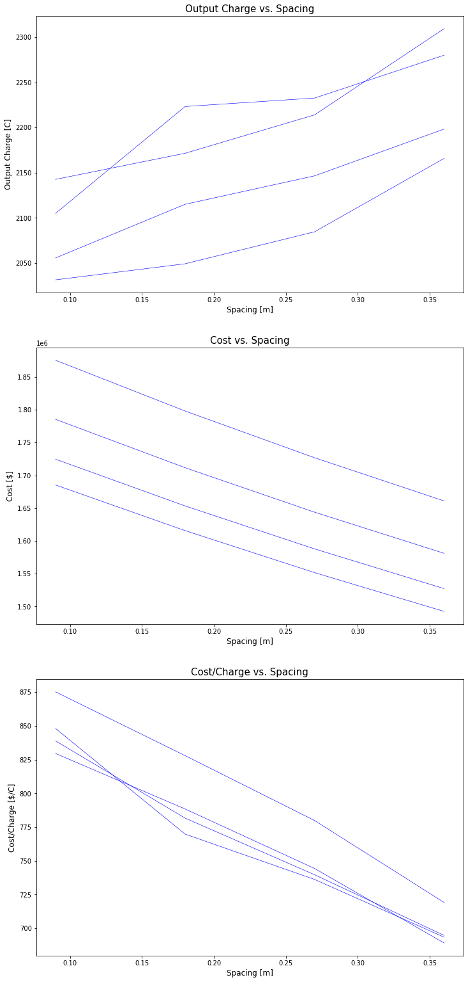
\includegraphics[width=3in]{fig31.png}
    \end{center}
    \renewcommand{\baselinestretch}{1}
    \small\normalsize
    \begin{quote}
    \caption[Batch 3 Spacing Trends]{Batch 3 Spacing Trends} \label{fig: f31}
    \end{quote}
\end{figure}

Having determined the output for the most economic configuration, we also obtained a value for the maximum output 
possible for the physical space in a highway setting. This value was 12334.1 C for 1600 m. 
We will use the selected charge outputs for the economical configuration and maximum output configuration to 
determine if this design can sustain an electric vehicle in the long term. 

See Figures \ref{fig: f32} and \ref{fig: f33} below for a visual representation of the most economical output and the maximum output configurations 
over 20 m.

\begin{figure}
    \begin{center}
    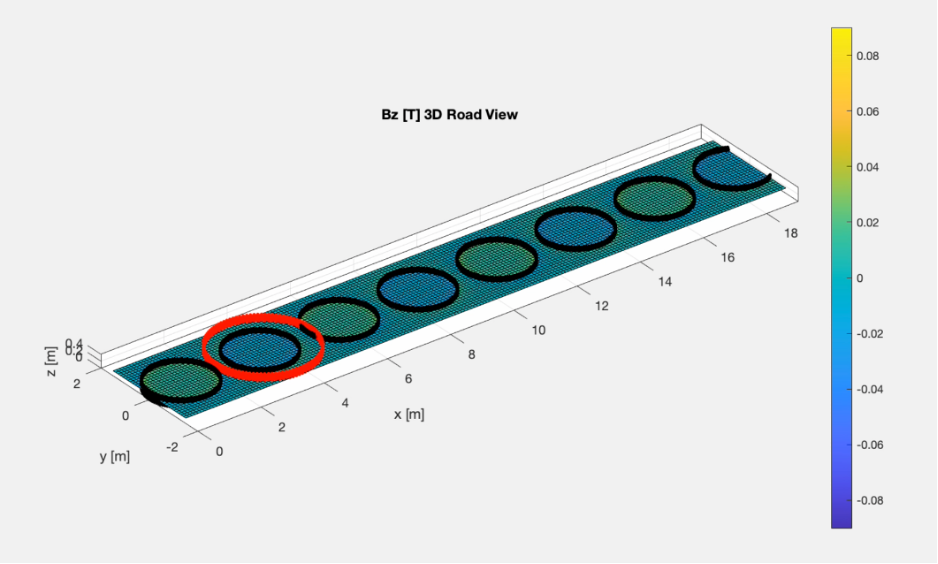
\includegraphics[width=5in]{fig32.png}
    \end{center}
    \renewcommand{\baselinestretch}{1}
    \small\normalsize
    \begin{quote}
    \caption[Economical Configuration Magnetic Field]{Economical Configuration Magnetic Field} \label{fig: f32}
    \end{quote}
\end{figure}

\begin{figure}
    \begin{center}
    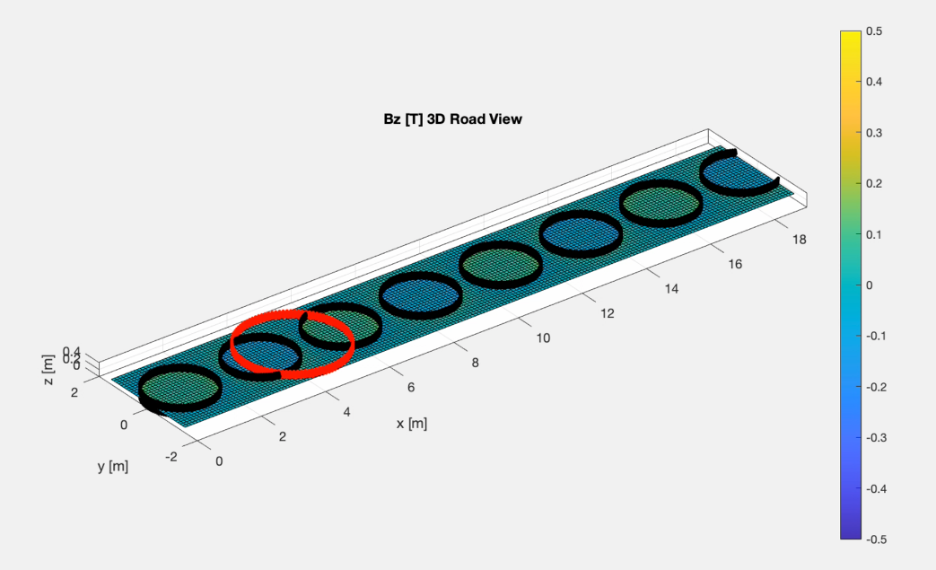
\includegraphics[width=5in]{fig33.png}
    \end{center}
    \renewcommand{\baselinestretch}{1}
    \small\normalsize
    \begin{quote}
    \caption[Maximum Output Configuration Magnetic Field]{Maximum Output Configuration Magnetic Field} \label{fig: f33}
    \end{quote}
\end{figure}

\section{Experimental Model}
Due to the circumstances surrounding COVID-19, results from in-person testing are delayed. For the purpose of 
this paper, the expected results will be discussed. As previously stated, the experimental model’s purpose 
is to provide a “real-world” comparison to the simulation results. Optimally, the data obtained through 
physical testing will validate the simulations and reinforce the variable relationships they produce.

The data from physical testing will be recorded using an oscilloscope which will yield voltage and current 
graphs pertaining to the receiving coil. The current graph will then be integrated with respect to time to 
obtain the cumulative charge acquired by the receiving coils. The modularity of the experimental model 
allows for variables such as transmitting coil current, spacing of the transmitting coils, height between 
the transmitting and receiving coils, and velocity of the receiving coil. The alteration of these variables 
will display their relationship with acquired charge. These relationships are then used to optimize the DWPT 
system to acquire the most charge. After multiple tests are run for the different variable scenarios, the 
testing team will plot the results and compare them with the plots produced by the simulations shown in 
Figures \ref{fig: f34} through \ref{fig: f37}.

\begin{figure}
    \begin{center}
    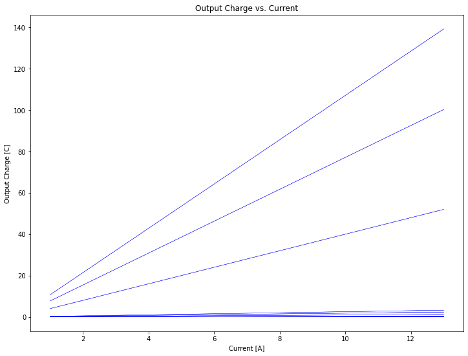
\includegraphics[width=3in]{fig34.png}
    \end{center}
    \renewcommand{\baselinestretch}{1}
    \small\normalsize
    \begin{quote}
    \caption[Experimental Model Expected Current Trend]{Experimental Model Expected Current Trend} \label{fig: f34}
    \end{quote}
\end{figure}

\begin{figure}
    \begin{center}
    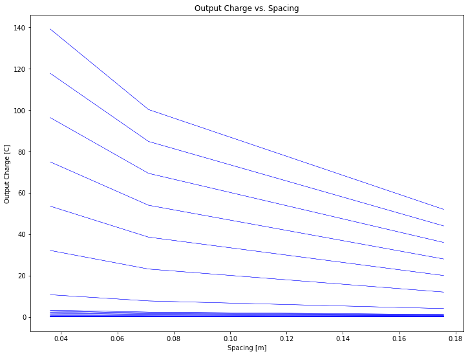
\includegraphics[width=3in]{fig35.png}
    \end{center}
    \renewcommand{\baselinestretch}{1}
    \small\normalsize
    \begin{quote}
    \caption[Experimental Model Expected Spacing Trend]{Experimental Model Expected Spacing Trend} \label{fig: f35}
    \end{quote}
\end{figure}

\begin{figure}
    \begin{center}
    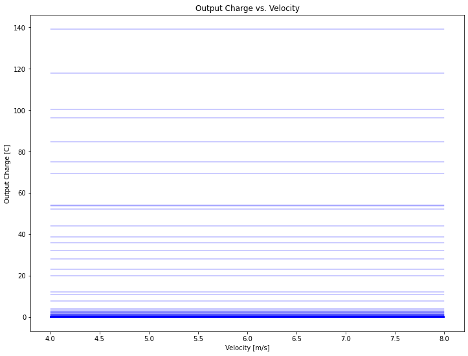
\includegraphics[width=3in]{fig36.png}
    \end{center}
    \renewcommand{\baselinestretch}{1}
    \small\normalsize
    \begin{quote}
    \caption[Experimental Model Expected Velocity Trend]{Experimental Model Expected Velocity Trend} \label{fig: f36}
    \end{quote}
\end{figure}

\begin{figure}
    \begin{center}
    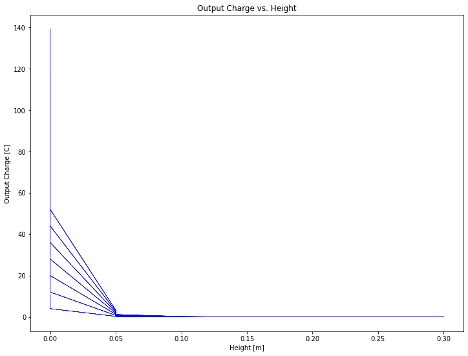
\includegraphics[width=3in]{fig37.png}
    \end{center}
    \renewcommand{\baselinestretch}{1}
    \small\normalsize
    \begin{quote}
    \caption[Experimental Model Expected Height Trend]{Experimental Model Expected Height Trend} \label{fig: f37}
    \end{quote}
\end{figure}

The comparison of the experimental model data and simulation data will reveal the accuracy of the current model. 
At first it is likely that the two data sets will deviate from each other due to unmodeled dynamics. 
The equations used to develop the model assume ideal conditions when that is not a likely scenario. 
After this, the iterative process of altering the model to better represent the experimental data begins. 